\documentclass[10pt]{article}

% amsmath package, useful for mathematical formulas
\usepackage{amsmath}
% amssymb package, useful for mathematical symbols
\usepackage{amssymb}

% graphicx package, useful for including eps and pdf graphics
% include graphics with the command \includegraphics
\usepackage{graphicx}

% cite package, to clean up citations in the main text. Do not remove.
\usepackage{cite}

\usepackage{color} 

% Use doublespacing - comment out for single spacing
%\usepackage{setspace} 
%\doublespacing


% Text layout
\topmargin 0.0cm
\oddsidemargin 0.5cm
\evensidemargin 0.5cm
\textwidth 16cm 
\textheight 21cm

% Bold the 'Figure #' in the caption and separate it with a period
% Captions will be left justified
\usepackage[labelfont=bf,labelsep=period,justification=raggedright]{caption}

% Use the PLoS provided bibtex style
\bibliographystyle{PLoS2009}

% Remove brackets from numbering in List of References
\makeatletter
\renewcommand{\@biblabel}[1]{\quad#1.}
\makeatother


% Leave date blank
\date{}

\pagestyle{myheadings}
%% ** EDIT HERE **
%% Please insert a running head of 30 characters or less.  
%% Include it twice, once between each set of braces
\markboth{Evolutionary modeling}{Evolutionary modeling}

%% ** EDIT HERE **
%% PLEASE INCLUDE ALL MACROS BELOW
\usepackage{setspace}
\doublespacing

%parsetree.sty - LaTeX style file with macros for typesetting parse trees
% See parsetree.doc for extensive section-by-section comments to the code.
% Eirik Hektoen, 1994-2-24

\typeout{Including style file `parsetree.sty'.}


% Some Initial Variables and Auxiliary Macros:

\def\pterror#1{\errmessage{Parsetree ERROR: #1}}

\newdimen\pthgap\def\pthorgap#1{\pthgap=#1}
\newdimen\ptvgap\def\ptvergap#1{\ptvgap=#1}

\newbox\ptnodestrutbox\def\ptnodestrut{\unhcopy\ptnodestrutbox}
\newbox\ptleafstrutbox\def\ptleafstrut{\unhcopy\ptleafstrutbox}

\def\ptnodefont#1#2#3{\def\ptnodefn{#1}
  \setbox\ptnodestrutbox=\hbox{\vrule height#2 width0pt depth#3}}
\def\ptleaffont#1#2#3{\def\ptleaffn{#1}
  \setbox\ptleafstrutbox=\hbox{\vrule height#2 width0pt depth#3}}


% Customizable Definitions (- NOTE: MAY BE REDEFINED IN DOCUMENT -):

\pthorgap{12pt}                         % horizontal gap betw sisters
\ptvergap{12pt}                         % vertical gap betw mother/daughter
\ptnodefont{\normalsize\rm}{11pt}{3pt}  % font and strut height/depth: nodes
\ptleaffont{\normalsize\it}{11pt}{3pt}  % font and strut height/depth: leaves


% Hierarchy-building macros:

\newcount\ptdepth           % current bracketing depth
\newcount\ptn               % 1: m, 2: ma, 3: mab, 4: mabc
\newbox\ptm \newdimen\ptmx  % m = mother
\newbox\pta \newdimen\ptax  % a = 1st daughter
\newbox\ptb \newdimen\ptbx  % b = 2nd daughter
\newbox\ptc \newdimen\ptcx  % c = 3rd daughter (max)
\newbox\ptx \newdimen\ptxx  % x = used for passing results
\newif\ifpttri              % choose triangular subtree with \pttritrue

\def\ptnext{\advance\ptn by 1 \ifcase\ptn
  \or \setbox\ptm=\box\ptx \ptmx=\ptxx \or \setbox\pta=\box\ptx \ptax=\ptxx
  \or \setbox\ptb=\box\ptx \ptbx=\ptxx \or \setbox\ptc=\box\ptx \ptcx=\ptxx
  \else \pterror{More than 3 daughters in (sub)tree}\fi}

\def\ptbegtree{\ptdepth=0}
\def\ptendtree
  {\ifnum\ptdepth>0 \pterror{Mismatched bracketing: too few ')'s!}\fi}

\def\ptbeg{\ifnum\ptdepth=0 \leavevmode\fi\begingroup
  \advance\ptdepth1 \ptn=0\pttrifalse}
\def\ptend{\ifnum\ptdepth=0 \pterror{Mismatched bracketing: too many ')'s!}
  \else\ptcons\endgroup\ifnum\ptdepth=0 \box\ptx\else\ptnext\fi\fi}

\def\ptnodeaux#1{\setbox\ptx=\hbox{#1}\ptxx=0.5\wd\ptx\ptnext}
\def\ptnode#1{\ptnodeaux{\ptnodefn\ptnodestrut #1}}
\def\ptleaf#1{\ptnodeaux{\ptleaffn\ptleafstrut #1}}

\def\pthoradjust#1{\ifcase\ptn
  \or \pthadjbox{\ptm}{#1} \or \pthadjbox{\pta}{#1}
  \or \pthadjbox{\ptb}{#1} \or \pthadjbox{\ptc}{#1}
  \else \pterror{More than 3 daughters in (sub)tree}\fi}
\def\pthadjbox#1#2{\setbox#1=\hbox{\box#1\kern#2}}


% Subtree-constructing macros:

\def\ptcons
 {\ifnum\ptn=0 \ptconsz 
  \else
    \ifpttri\ptconstri\else
      \ifcase\ptn \or\ptconsm\or\ptconsma\or\ptconsmab\or\ptconsmabc \fi \fi
    \ptax=\ptxx \advance\ptax-\ptmx \ptbx=0pt
    \ifdim\ptax<0pt \ptbx=-\ptax\ptax=0pt\ptxx=\ptmx \fi
    \setbox\ptx=\vtop{\hbox{\kern\ptax\box\ptm}\nointerlineskip
                      \hbox{\kern\ptbx\box\ptx}}\fi
  \global\ptxx=\ptxx\global\setbox\ptx=\box\ptx}

\def\ptavg#1#2#3{#1=#2\advance#1#3#1=0.5#1}     % #1 := average(#2,#3)
\def\ptadv#1#2{\advance#1#2\advance#1\pthgap}   % #1 := #1 + #2 + \pthgap

\def\ptconsz{\ptxx=0pt \setbox\ptx=\vtop{}}     % empty (zero) tree

\def\ptconsm{\ptxx=0pt 
  \setbox\ptx=\hbox{\ptedge{1}{0}{}{}}}         % mother only

\def\ptconsma                                   % mother and one daughter
 {\ptxx=\ptax\setbox\ptx=\vtop{
    \hbox{\ptedge{1}\ptax{}{}}\nointerlineskip
    \hbox{\box\pta}}}

\def\ptconsmab                                  % mother and two daughters
 {\ptadv\ptbx{\wd\pta}\ptavg\ptxx\ptax\ptbx
  \setbox\ptx=\vtop{
    \hbox{\ptedge{2}\ptax\ptbx{}}\nointerlineskip
    \hbox{\box\pta\kern\pthgap\box\ptb}}}

\def\ptconsmabc                                 % mother and three daughters
 {\ptadv\ptbx{\wd\pta}\ptadv\ptcx{\wd\pta}%
  \ptadv\ptcx{\wd\ptb}\ptavg\ptxx\ptax\ptcx
  \setbox\ptx=\vtop{
    \hbox{\ptedge{3}\ptax\ptbx\ptcx}\nointerlineskip
    \hbox{\box\pta\kern\pthgap\box\ptb\kern\pthgap\box\ptc}}}

\def\ptconstri                                  % triangular subtree
 {\ifcase\ptn\or\setbox\pta\hbox{\kern2\pthgap}\or
  \or\setbox\pta=\hbox{\box\pta\kern\pthgap\box\ptb}
  \or\setbox\pta=\hbox{\box\pta\kern\pthgap\box\ptb\kern\pthgap\box\ptc}\fi
  \ptxx=0.5\wd\pta
  \setbox\ptx=\vtop{
    \hbox{\ptedge{0}{0}{\wd\pta}{}}\nointerlineskip
    \box\pta}}


% Macros for `diagonal rules':

\newcount\pted          % edge mode
\newcount\ptedm         % position of mother
\newcount\pteda         % position a
\newcount\ptedb         % position b
\newcount\ptedc         % position c
\newcount\ptedl         % edge length
\newcount\ptedh         % edge height
\newcount\ptedhs        % horizontal slope
\newcount\ptedvs        % vertical slope
\newcount\ptedtemp      % temporary variable

\def\ptedge#1#2#3#4{\pted=#1%
  \pteda=#2\ifcase\pted\ptedb=#3\or\or\ptedb=#3\or\ptedb=#3\ptedc=#4\fi
  \ptedm=\pteda\advance\ptedm\ifcase\pted\ptedb\or\pteda\or\ptedb\or\ptedc\fi
  \divide\ptedm by 2
  \ptedh=\ptvgap\ptedtemp=\ptedm\advance\ptedtemp-\pteda\divide\ptedtemp by 6
  \ifnum\ptedh<\ptedtemp\ptedh=\ptedtemp\fi
  \unitlength=1sp%
  \begin{picture}(0,\ptedh)
    \ifnum\pted=3 \ptedput\ptedc\fi
    \ifnum\pted=1 \else\ptedput\ptedb\fi
    \ptedput\pteda
    \ifnum\pted=0 \ptedbot\fi 
  \end{picture}}

\def\ptedput#1{\ptedl=#1\advance\ptedl-\ptedm
  \ifnum\ptedl>0 \ptedslope\else
    \ptedl=-\ptedl\ptedslope\ptedhs=-\ptedhs\fi
  \ifnum\ptedhs=0 \ptedl=\ptedh\fi
  \put(\ptedm,\ptedh){\line(\ptedhs,-\ptedvs){\ptedl}}}

\def\ptedbot
 {\ptedtemp=\ptedl\multiply\ptedtemp by \ptedvs\divide\ptedtemp by \ptedhs
  \ifnum\ptedtemp>0\ptedtemp=-\ptedtemp\fi \advance\ptedtemp-1
  \advance\ptedtemp\ptedh\multiply\ptedl by 2
  \put(\pteda,\ptedtemp){\line(1,0){\ptedl}}}

\def\ptedslope
 {\ifnum\ptedl>\ptedh\ptedhs=\ptedl\ptedvs=\ptedh
  \else              \ptedvs=\ptedl\ptedhs=\ptedh \fi
  \divide\ptedhs by 60 \divide\ptedvs by \ptedhs
  \ifnum \ptedvs <  5 \ptedvs=0 \ptedhs=1 \else
  \ifnum \ptedvs < 11 \ptedvs=1 \ptedhs=6 \else
  \ifnum \ptedvs < 13 \ptedvs=1 \ptedhs=5 \else
  \ifnum \ptedvs < 17 \ptedvs=1 \ptedhs=4 \else
  \ifnum \ptedvs < 22 \ptedvs=1 \ptedhs=3 \else
  \ifnum \ptedvs < 27 \ptedvs=2 \ptedhs=5 \else
  \ifnum \ptedvs < 33 \ptedvs=1 \ptedhs=2 \else
  \ifnum \ptedvs < 38 \ptedvs=3 \ptedhs=5 \else
  \ifnum \ptedvs < 42 \ptedvs=2 \ptedhs=3 \else
  \ifnum \ptedvs < 46 \ptedvs=3 \ptedhs=4 \else
  \ifnum \ptedvs < 49 \ptedvs=4 \ptedhs=5 \else
  \ifnum \ptedvs < 55 \ptedvs=5 \ptedhs=6 \else
                      \ptedvs=1 \ptedhs=1 
    \fi \fi \fi \fi \fi \fi \fi \fi \fi \fi \fi \fi
  \ifnum \ptedl < \ptedh
    \ptedtemp=\ptedhs \ptedhs=\ptedvs \ptedvs=\ptedtemp \fi}


% Convenient End-User Environment:

\newenvironment{parsetree}{\ptactivechardefs\ptbegtree}{\ptendtree}

\def\ptcatcodes
 {\catcode`(=\active \catcode`)=\active
  \catcode`.=\active \catcode``=\active
  \catcode`~=\active}

{\ptcatcodes
\gdef\ptactivechardefs
 {\ptcatcodes
  \def({\ptbeg\ignorespaces}
  \def){\ptend\ignorespaces}
  \def.##1.{\ptnode{##1}\ignorespaces} 
  \def`##1'{\ptleaf{##1}\ignorespaces}
  \def~{\pttritrue\ignorespaces}}}



% to link empty nodes
%\def\ptlink{\rule{0.4pt}{\ht\ptnodestrutbox + \dt\ptnodestrutbox}}
\def\ptlink{\vrule height\ht\ptnodestrutbox depth\dp\ptnodestrutbox}





\newcommand\titlestring{Evolutionary triplet models of structured RNA}
\newcommand\authorstring{
Robert K. Bradley$^{1}$, 
Ian Holmes$^{1,2,\ast}$
\\
\textbf{1} Biophysics Graduate Group, University of California, Berkeley, CA, USA
\\
\textbf{2} Department of Bioengineering, University of California, Berkeley, CA, USA
\\
$\ast$ E-mail: indiegram@postbox.biowiki.org
}

\usepackage{array}

\usepackage[boxed]{algorithm2e}
\usepackage{mathrsfs}

% Labels & references for sections, figures and tables
% Commented out \secref definition & replaced \seclabel with a dummy, because PLoS doesn't like numbered section references -- IH, 11/11/08
% (This edit appears to have been reversed as of 5/29/09 - presumably so that the supplementary information compiles OK using these same definitions - IH, 5/29/09)
\newcommand{\secref}[1]{Section~\ref{sec:#1}}
\newcommand{\seclabel}[1]{\label{sec:#1}}

\newcommand{\secname}[1]{``#1''}  % PLoS-style section names

% "Text S1"
\newcommand{\supptext}[1]{Text S#1}

\newcommand{\appref}[1]{Appendix~\ref{app:#1}}
\newcommand{\applabel}[1]{\label{app:#1}}

\newcommand{\figref}[1]{Figure~\ref{fig:#1}}
\newcommand{\figlabel}[1]{\label{fig:#1}}

\newcommand{\tabnum}[1]{\ref{tab:#1}}
\newcommand{\tabref}[1]{Table~\tabnum{#1}}
\newcommand{\tablabel}[1]{\label{tab:#1}}

\newcommand{\algref}[1]{Algorithm~\ref{alg:#1}}
\newcommand{\alglabel}[1]{\label{alg:#1}}

\newcommand{\eqnref}[1]{Equation~\ref{eqn:#1}}
\newcommand{\eqnlabel}[1]{\label{eqn:#1}}

% Frequently used proper nouns that should have consistent typeface, capitalization, etc.
\newcommand{\pfold}{PFOLD}
\newcommand\darturl{{\tt http://biowiki.org/dart}}
\newcommand\indiegramurl{{\tt http://biowiki.org/IndieGram}}
\newcommand{\dart}{DART}

\newcommand{\bralibaseII}{BRalibaseII}
\newcommand{\balibase}{BAliBASE}

\newcommand{\stemloc}{Stemloc}
\newcommand{\stemlocama}{Stemloc-AMA}
\newcommand{\xrate}{XRate}
\newcommand{\evoldoer}{Evoldoer}
\newcommand{\evolsayer}{{\tt evolsayer.pl}}
\newcommand{\animateevolsayer}{{\tt animate-evolsayer.pl}}
\newcommand{\indiegram}{Indiegram}
\newcommand{\handel}{Handel}

\newcommand{\contrafold}{CONTRAFOLD}
\newcommand{\consan}{CONSAN}
\newcommand{\clustalw}{ClustalW}
\newcommand{\foldalign}{Foldalign}
\newcommand{\foldalignm}{FoldalignM}
\newcommand{\mastr}{MASTR}
\newcommand{\rnasampler}{RNASampler}
\newcommand{\murlet}{Murlet}
\newcommand{\ortheus}{Ortheus}
\newcommand{\rnaalifold}{RNAAlifold}
\newcommand{\viennarna}{ViennaRNA}

\newcommand{\RFAM}{RFAM}

\newcommand{\denovo}{{\em de novo}}

\newcommand{\nth}{\mathrm{n}^{\mathrm{th}}}
\newcommand{\mth}{\mathrm{m}^{\mathrm{th}}}

\newcommand{\type}[0]{\operatorname{type}}
\newcommand{\emit}[0]{\operatorname{emit}}
\newcommand{\absorb}[0]{\operatorname{absorb}}
\newcommand{\argmax}[0]{\operatorname{argmax}}
\newcommand{\argmin}[0]{\operatorname{argmin}}
\newcommand{\parent}[0]{\operatorname{parent}}

\newcommand{\weight}[0]{\operatorname{Weight}}
\newcommand{\transweight}[3]{t\left(#2,#3|\theta^{(#1)}\right)}  % {m}{from}{to}
\newcommand{\emissionweight}[3]{e_{#2}\left(#3|\theta^{(#1)}\right)}  % {m}{emitstate}{emission}
\newcommand{\totalemissionweight}[2]{\mathbb{e}_{#1}(#2)}

%\newcommand{\cyk}[7]{\gamma_{#1}(#2,#3,#4,#5,#6,#7)}
\newcommand{\cyk}[7]{\gamma_{#1}\left(#2,#3,#4\right)}
%\newcommand{\cyk}[7]{\gamma_{#1}(#2,#3,#4)}
%\newcommand{\inside}[7]{\alpha_{#1}(#2,#3,#4,#5,#6,#7)}
\newcommand{\inside}[7]{\alpha_{#1}\left(#2,#3,#4\right)}
%\newcommand{\outside}[7]{\beta_{#1}(#2,#3,#4,#5,#6,#7)}
\newcommand{\outside}[7]{\beta_{#1}\left(#2,#3\right,#4\right)}

\newcommand{\Tnull}{\mathrm{null}}
\newcommand{\Tgap}{\mathrm{GAP}}

\newcommand{\statetype}[1]{\mathtt{#1}}
\newcommand{\state}[3]{{}^{#2}\mathtt{#1}^{#3}}
% Note that this will only work for left-bifurcations!
%\newcommand{\bifurc}[3]{{\phantom{]}}^{#2}\mathtt{B[#3\,#1]}}}
\newcommand{\bifurc}[3]{\mathtt{#1[#2\,#3]}}

% state types for branch transducers
\newcommand{\Sstart}[0]{\statetype{Start}}
\newcommand{\Smatch}[0]{\statetype{Match}}
\newcommand{\Sinsert}[0]{\statetype{Insert}}
\newcommand{\Swait}[0]{\statetype{Wait}}
\newcommand{\Send}[0]{\statetype{End}}

% state types for evolutionary model
\newcommand{\Snull}[0]{\statetype{Null}}
\newcommand{\Sbifurc}[0]{\statetype{Bifurcation}}
\newcommand{\Semit}[0]{\statetype{Emit}}

\newcommand{\statevec}[1]{\left(\begin{array}{c}#1_1\\\vdots\\#1_N\end{array}\right)}
\newcommand{\fourvec}[4]{\left(\begin{array}{c}#1\\#2\\#3\\#4\end{array}\right)}
\newcommand{\nakedfourvec}[4]{\begin{array}{c}#1\\#2\\#3\\#4\end{array}}
\newcommand{\threevec}[3]{\left(\begin{array}{c}#1\\#2\\#3\end{array}\right)}
\newcommand{\nakedthreevec}[3]{\begin{array}{c}#1\\#2\\#3\end{array}}
\newcommand{\bvec}[1]{\boldsymbol{#1}}
\newcommand{\activenode}[1]{n(\bvec{#1})}

\newcommand{\foldenv}{\mathscr{F}}

\newcommand{\mDn}[0]{m \vartriangleright n}
\newcommand{\mNDn}[0]{m \ntriangleright n}
\newcommand{\mDEn}[0]{m \trianglerighteq n}
\newcommand{\mNDEn}[0]{m \ntrianglerighteq n}


\newcommand{\beqn}{\begin{equation}}
\newcommand{\eeqn}{\end{equation}}







\newcommand\gnons{{\cal N}}
\newcommand\gnulls{{\bf N}}
\newcommand\gbifs{{\bf B}}
\newcommand\gemits{{\bf E}}
\newcommand\gterms{\Omega}
\newcommand\grules{{\bf R}}
\newcommand\grhs{( \gnons \cup \Omega )^\ast}
\newcommand\gtrees{{\cal T}}

\newcommand\leftside[1]{{\cal L}(#1)}
\newcommand\rightside[1]{{\cal R}(#1)}
\newcommand\allrules[1]{{\cal A}(#1)}




\newcommand\revisionnotes
{\noindent \hrulefill{} \\ {\bf Revision Notes:}
\begin{enumerate}
\item These comments are not a complete summary of the review, just a partial strategy for addressing some of the points.
The review is the more authoritative guide...
He is giving us the benefit of the doubt but acceptance is still very much in the balance, I think, so we need to stick at it,
and take it that extra step beyond minimal compliance with his suggestions.
%
\item Obviously we have to do simulation tests and hopefully EvolSayer will be of some use there.
One thing to be careful of is that there are certain regimes of rate/branch-length parameter space where the ``trivial'' outcomes identified by the reviewer
(ancestral sequence is always identical to one of the descendants) are the norm.
Oscar and I have been looking at this quite a bit recently (see also 2003 paper by Mossel).
The regime we are probably most interested in is where the branch lengths are of comparable length
and so the two slightly-longer branches can ``out-vote'' the shorter branch under certain conditions.
This should probably be commented on in the paper: the reviewer says he would be happy with ``a small, noncomprehensive set of anecdotes''
but if we can rationalize why some parameter settings are more interesting than others, then that's all to the better.
%
\item I would actually be very wary of taking that ``small noncomprehensive set of anecdotes'' at face value.
This is one area where I sense we're being given enough rope to hang ourselves... an unsatisfactory response to the simulation issue will be unequivocal grounds for rejection.
Obviously there are limits to the number of simulations we can run, but with EvolSayer's output statistics (allowing us to filter out ``interesting'' cases), we can automate it somewhat.
%
\item I wrote out the TKF structure tree for the case $a \to b \to c$,
which can be used to estimate the intermediate sequence $b$
(e.g. for Redelings-Suchard).
I think this could be useful in explaining tree transducer composition more concretely, and why is important:
by inspecting these tables, the reader can see that the structure of this grammar is quite complicated,
and should then be prepared for the idea that the ``composition algorithm'' is simply generating this table
(or other tables for other phylogenies).
The latex for this is in the file ``tkfst.tex'', and is currently include'd at the start of the supplementary information (it should go in the main paper though, I think).
%
\item Can we dump out the grammar for the three-branch TKFST and include it in the Supplement?
(Or the main paper?) I realize it's huge, but this very hugeness does motivate the transducer composition algorithm,
in the same way that the two-branch model (which is now included in a more human-readable form) does.
%
\item If we are moving the description of loopy DP to the main paper, I think it needs to be more precise.
Currently it just says ``we repeatedly iterate over strongly-connected components of the state sub graph'',
which falls short of the level of precision/detail with which the other DP algorithms are presented.
The description should encompass alternate strategies (i.e. orders of visiting the states) that you have considered:
randomized, Tarjan's algorithm, etc.
The reader should be left understanding the pros-and-cons of each,
 e.g. worst-case performance or difficulty of implementation.
No need to agonize about this, but be helpful to potential future developers.
  (Example reader: a grad student in our group who might try to implement loopy DP themselves.)
%
\item The descriptions of the DP algorithms do not currently include any traceback algorithms (CYK or Inside);
therefore, we haven't technically described how to do ancestral reconstruction!
Obviously these algorithms are almost trivial, but they're quite important.
Implementing stochastic loopy-Inside traceback in tripletscfgdp.\{h,cc\} is a key step in transforming it into a useful tool
(for example, with this extension, Indiegram would be pretty much ready-to-go for Redelings-Suchard sampling).
The deterministic CYK traceback algorithm is {\em even more} important to present here, because implementing this algorithm is currently our main result!
The paper should describe {\em both} these traceback algorithms.
This shouldn't be that hard to do in a comprehensible, rigorous style
 (loopy traceback is much simpler than the algorithms for restoring eliminated states to traceback paths, which are painfully described in my 2003 paper).
%
\item All algorithms should be described in full, rather than giving recipes for deriving some algorithms from others.
In particular, the CYK algorithm is currently summarized by statements along the lines of
``replace sums over paths through the model (or equivalently, parses) with the $\max()$ operation (e.g., in equation X, sum-over-complicated-expression will be replaced with max-over-complicated-expression)''.
It shouldn't be too hard to write a latex command/macro that can be used (with ``$\sum$'' or ``$\max$'' as an argument) to generate complete versions of {\em both} algorithms.
%
\item The paper the reviewer cites as an example of the simplicity of missing data estimation (Rivas and Eddy (2008) PLoS CB 4:e1000172) is an IID-columns model for a multiple alignment.
When he says that this issue ``may simply go away if you view the problem as a missing data problem'',
that is precisely what we are talking about when we discuss null cycle elimination.
I've tried to explain in ``tkfst.tex'' why this is harder than it superficially appears:
\begin{enumerate}
\item eliminating missing ``empty'' columns from an IID-columns model (such as in Rivas and Eddy, 2008) is easy.
\item eliminating missing emissions from an HMM is slightly harder (c.f. ``wing retraction'' algorithm in HMMer source code)
but general algorithms do exist.
\item eliminating null states from an SCFG is much harder, due to null bifurcations.
\end{enumerate}
%
\item The reviewer asks for early discussion of constraints in the context of the ``rate-limiting steps of paleogenetics''.
We should take this opportunity to clarify that our approach is (1) formulate the model,  (2) apply appropriate constraints.
Our emphasis here is on (1).
Cite the literature: QRNA represents an alignment constraint on a pair SCFG, Holmes-Rubin 2002 uses fold constraints on pair SCFGs,
stemloc uses fold+alignment constraints, Ortheus uses an alignment constraint, etc, but none of these things can be done
(in a probabilistic modeling framework at least) until you can formulate the model.
For this paper, we chose to condition on structures essentially because they are easy to constrain
(fold envelopes can be applied independently to each sequence).
But we could equally easily have conditioned on alignments. Constraints are easy to tweak, once you have a model.
%
\item The reviewer also comments on the phylogeny being a given.
We can note that even though we constrain the phylogeny, more realistic phylogenetic applications are possible.
Given a structural phylo-alignment (tree+alignment+structure), we can calculate the likelihood; therefore, given two such structural phylo-alignments,
we can say which one is more probable (describe their relative posterior probabilities, etc.).
From this it is possible to make a crude MCMC sampler, just by proposing/accepting/rejecting alignment/tree/structure changes.
An {\em efficient} MCMC sampler needs to be able to make local topology changes and to resample the multiple alignment around a topology change;
we can do this too, in principle, but it's beyond this paper.
%
\item As I understand it, pruning \& peeling are not exactly equivalent as the reviewer claims, {\em except} in the special case of a reversible model.
Specifically, pruning is a {\em restricted case} of peeling, giving you the posterior probabilities at the root node, but not any other node.
Of course, if you have a reversible model, you can re-root the tree anywhere, and so the two are equivalent for reversible models only.
When Felsenstein says the two approaches are the same (on p253 of his book), it is quite a vague statement:
e.g. later in the same paragraph, he says that both peeling and pruning are variants of Horner's rule, and particular cases of dynamic programming.
All of this is somewhat academic; basically I'm thinking the pruning/peeling distinction might yet have some pedagogic value, and we might not need to abandon it entirely.
%
\item We should address all the reviewer's comments about the figures if possible.
I have added xfig files ``stree.fig'' and ``stree-mutations.fig'' to the repository; the latter shows an evolutionary trajectory of the TKFST, as requested by the reviewer.
%
\item Finally, a very minor/trivial point: would you consider a name-change for IndieGram to something beginning with ``Evol''?
The EvolDeeds package is EvolDoer (previously released as ``tkfstalign''), EvolSayer and IndieGram.
I put a few random suggestions for Evol-names at {\bf biowiki.org/EvolDeeds}.
Don't take this too seriously, of course!
I'll understand if you want to stick with IndieGram, and this is obviously negligible compared to the other revisions.
%
\end{enumerate}
\hrulefill{}}


% no idea why \outside was redefined with a "\right," instead of a normal comma in defs.tex, but am redefining it back here - IH, 5/29/09
\renewcommand{\outside}[7]{\beta_{#1}\left(#2,#3,#4\right)}
%% END MACROS SECTION

\begin{document}

% Title must be 150 words or less
\begin{flushleft}
  {\Large
    \textbf{\titlestring: \supptext{4}}
  }
\\
\authorstring
\end{flushleft}

\newpage
\section{Inference grammars for the TKFST model}
\seclabel{TKFST}

This section describes multi-sequence grammars that can be used to infer alignments, structures and ancestors under the
TKF Structure Tree (TKFST) model.

% TKF Structure Tree: Pair SCFGs & parameterizations.
% Summarized from rnaevol-paper/rnaevol.tex  by IH, 12/9/2008

\newcommand\gap{\ast}

\newcommand\ruletable[3]{
\begin{tabular}{rcc|rrr}
\multicolumn{6}{l}{\em #1} \\
\multicolumn{6}{l}{\em #2}\\
#3
\end{tabular}
}
\newcommand\tkfstruletable[3]{\ruletable{TKF Structure Tree #1}{#2}{#3}}

\newcommand\lhsrhs[5]{ #1 & $\to$ & #2 & #3 & #4 & #5 \\ }
\newcommand\rhs[4]{       &   $|$ & #1 & #2 & #3 & #4 \\ }
\newcommand\blank{ & & & & & \\ }


\newcommand\singletgrammar[3]{
% #1 = tree node identifier
% #2 = 5' terminal (left)
% #3 = 3' terminal (right)
\tkfstruletable{singlet rules ($#1$)}
{Sequence $#1$ terminals: $\{ #2, #3 \}$.}
{
\lhsrhs{ lhs }{ rhs }{ $P(#1)$ }{  }{  }
\hline

\blank
\lhsrhs{ $L_{#1}$ }{ ${#2}\ L_{#1}$ }{ $\kappa_l \pi_l(#2)$ }{  }{  }
\rhs{ $S_{#1}\ L_{#1}$ }{ $\kappa_l \pi_l(S)$ }{  }{  }

\rhs{ $\epsilon$ }{ $1-\kappa_l$ }{  }{  }

\blank
\lhsrhs{ $S_{#1}$ }{ ${#2}\ S_{#1}\ {#3}$ }{ $\kappa_s \pi_s(#2#3)$ }{  }{  }
\rhs{ $L_{#1}$ }{ $1-\kappa_s$ }{  }{  }
}
}  % end \singletgrammar



\newcommand\pairgrammar[7]{
% #1 = ancestor
% #2 = descendant
% #3 = ancestral 5' terminal (left)
% #4 = ancestral 3' terminal (right)
% #5 = descendant 5' terminal (left)
% #6 = descendant 3' terminal (right)
% #7 = time suffix (empty string "", apostrophe "'", branch superscript "^{...}")
\tkfstruletable{pair rules ($#1 \stackrel{t#7}{\to} #2$)}
{Sequence $#1$ terminals: $\{ #3, #4 \}$. \quad  Sequence $#2$ terminals: $\{ #5, #6 \}$.}
{
\lhsrhs{ lhs }{ rhs }{ $P(#1)$ }{ $P(#2|#1)$ }{  }
\hline

\blank
\lhsrhs{ $L_{#1#2}$ }{ ${#3}\ {#5}\ L_{#1#2}$ }{ $\kappa_l \pi_l(#3)$ }{ $(1-\beta#7_l) \alpha#7_l M#7_l(#3,#5)$ }{  }
\rhs{ ${#5}\ L_{#1#2}$ }{ $1$ }{ $\beta#7_l \pi_l(#5)$ }{  }
\rhs{ ${#3}\ L_{#1\gap #2}$ }{ $\kappa_l \pi_l(#3)$ }{ $(1-\beta#7_l) (1-\alpha#7_l)$ }{  }

\blank
\rhs{ $S_{#1#2}\ L_{#1#2}$ }{ $\kappa_l \pi_l(S)$ }{ $(1-\beta#7_l) \alpha#7_l$ }{  }
\rhs{ $S_{#2}\ L_{#1#2}$ }{ $1$ }{ $\beta#7_l \pi_l(S)$ }{  }
\rhs{ $S_{#1}\ L_{#1\gap #2}$ }{ $\kappa_l \pi_l(S)$ }{ $(1-\beta#7_l) (1-\alpha#7_l)$ }{  }

\rhs{ $\epsilon$ }{ $1-\kappa_l$ }{ $1-\beta#7_l$ }{  }

\blank
\lhsrhs{ $S_{#1#2}$ }{ ${#3}\ {#5}\ S_{#1#2}\ {#6}\ {#4}$ }{ $\kappa_s \pi_s(#3#4)$ }{ $(1-\beta#7_s)  \alpha#7_s M#7_s(#3#4,#5#6)$ }{  }
\rhs{ ${#5}\ S_{#1#2}\ {#6}$ }{ $1$ }{ $\beta#7_s \pi_s(#5#6)$ }{  }
\rhs{ ${#3}\ S_{#1\gap #2}\ {#4}$ }{ $\kappa_s \pi_s(#3#4)$ }{ $(1-\beta#7_s) (1-\alpha#7_s)$ }{  }
\rhs{ $L_{#1#2}$ }{ $1-\kappa_s$ }{ $1-\beta#7_s$ }{  }

\blank
\lhsrhs{ $L_{#1\gap #2}$ }{ ${#3}\ {#5}\ L_{#1#2}$ }{ $\kappa_l \pi_l(#3)$ }{ $(1-\gamma#7_l) \alpha#7_l M#7_l(#3,#5)$ }{  }
\rhs{ ${#5}\ L_{#1#2}$ }{ $1$ }{ $\gamma#7_l \pi_l(#5)$ }{  }
\rhs{ ${#3}\ L_{#1\gap #2}$ }{ $\kappa_l \pi_l(#3)$ }{ $(1-\gamma#7_l) (1-\alpha#7_l)$ }{  }

\blank
\rhs{ $S_{#1#2}\ L_{#1#2}$ }{ $\kappa_l \pi_l(S)$ }{ $(1-\gamma#7_l) \alpha#7_l$ }{  }
\rhs{ $S_{#2}\ L_{#1#2}$ }{ $1$ }{ $\gamma#7_l \pi_l(S)$ }{  }
\rhs{ $S_{#1}\ L_{#1\gap #2}$ }{ $\kappa_l \pi_l(S)$ }{ $(1-\gamma#7_l) (1-\alpha#7_l)$ }{  }

\rhs{ $\epsilon$ }{ $1-\kappa_l$ }{ $1-\gamma#7_l$ }{  }

\blank
\lhsrhs{ $S_{#1\gap #2}$ }{ ${#3}\ {#5}\ S_{#1#2}\ {#6}\ {#4}$ }{ $\kappa_s \pi_s(#3#4)$ }{ $(1-\gamma#7_s) \alpha#7_s M#7_s(#3#4,#5#6)$ }{  }
\rhs{ ${#5}\ S_{#1#2}\ {#6}$ }{ $1$ }{ $\gamma#7_s \pi_s(#5#6)$ }{  }
\rhs{ ${#3}\ S_{#1\gap #2}\ {#4}$ }{ $\kappa_s \pi_s(#3#4)$ }{ $(1-\gamma#7_s) (1-\alpha#7_s)$ }{  }
\rhs{ $L_{#1#2}$ }{ $1-\kappa_s$ }{ $1-\gamma#7_s$ }{  }
}
}  % end \pairgrammar




\newcommand\abc{$a \stackrel{t}{\to} b \stackrel{t'}{\to} c$}
\newcommand\ab{$a \stackrel{t}{\to} b$}
\newcommand\bc{$b \stackrel{t'}{\to} c$}
\newcommand\ac{$a \stackrel{t+t'}{\longrightarrow} c$}

\newcommand\agapbc{a\gap bc}
\newcommand\abgapc{ab\gap c}

\newcommand\abcstates{``$abc$'' states (post emission at $c$)}
\newcommand\abgapcstates{``$\abgapc$'' states (post deletion on \bc\ branch)}
\newcommand\agapbcstates{``$\agapbc$'' states (post deletion on \ab\ branch)}




\subsection*{The TKFST model on a two-branch phylogeny}

While the idea of composing conditionally-normalized models on a tree
is intuitive, the resulting models can quickly become too complex to
deal with by hand, necessitating an algorithm for automated model
construction.  We constructed the model corresponding to TKFST on the
simple the two-branch phylogeny \abc.
The results, shown below, make clear that by-hand model construction
quickly becomes impractical as model complexity or tree size
increases.

We explicitly note cases where certain sets of grammar rules can be derived
``automatically'' from simpler sets, motivating the development of our
generic tree transducer composition algorithm.


\subsubsection*{Time-dependent probabilities}

Here $n \in \{ l, s \}$ denotes the type of structural element (loop or stem).
${\bf R}^{(n)}$ is the rate matrix and $\pi_n$ the equilibrium distribution.
$\lambda_n$ is the insertion rate and $\mu_n$ is the deletion rate.

\begin{eqnarray*}
\alpha_n(t) & = & \exp (-\mu_n t) \\
\beta_n(t)  & = & \frac {\lambda_n (1 - \exp((\lambda_n-\mu_n)t))} {\mu_n - \lambda_n \exp((\lambda_n-\mu_n)t)} \\
\gamma_n(t) & = & 1 - \frac {\mu_n (1 - \exp((\lambda_n-\mu_n)t))} {(1 - \exp(-\mu_n t))(\mu_n - \lambda_n \exp((\lambda_n-\mu_n)t))}\\
\kappa_n(t) & = & \lambda_n / \mu_n \\
M_n(i,j;t)  & = & \exp({\bf R}^{(n)} t)_{ij}
\end{eqnarray*}

Let $\alpha_n \equiv \alpha_n(t)$ and $\alpha'_n = \alpha_n(t')$; similarly $\beta'_n,\gamma'_n,M'_n$.

\subsubsection*{Grammars}

Note that any of the grammars can be ``downsized'' to a smaller number of sequences, simply by dropping terminals,
yielding alternative applications for each grammar.

For example, the Pair SCFG for \ab\ becomes a Single SCFG for $a$ if sequence $b$ is dropped by removing terminals $w,x$.
Stochastic traceback then can be used to sample the descendant $b$.
This corresponds to a forward-time simulator when we apply the Inside
\& stochastic traceback algorithms.

Similarly, \abc\ can be viewed as a pair grammar \ac\ that can be used
to sample an unknown evolutionary intermediate $b$. Again, this
requires only the Inside \& stochastic traceback algorithms.

% singlet grammars
\paragraph{Singlet rules.}

This section contains three singlet grammars, one for each of the sequences $a$, $b$ and $c$.

Note that Tables~\tabnum{b} and~\tabnum{c} may be deduced automatically from Table~\tabnum{a}
if it is known that the underlying process is initially at equilibrium.

\paragraph{Pair rules.}
% pair grammars

This section contains two pairwise rule-sets.

The pair grammar for \ab\ is the union of Tables~\tabnum{a}, \tabnum{b} and~\tabnum{ab}.

The pair grammar for \bc\ is the union of Tables~\tabnum{b}, \tabnum{c} and~\tabnum{bc}.


Note that \tabref{bc} may be deduced automatically from \tabref{ab}
if it is known that the underlying process is stationary.


\paragraph{Triplet rules.}
% triplet grammar

Because of its length, we have split the triplet rule-set over three tables:
\begin{description}
\item[\tabref{abc}:] Rules for transforming $\{ L_{abc}, S_{abc}\}$ , after emissions to $c$;
\item[\tabref{abgapc}:] Rules for transforming $\{ L_{\abgapc}, S_{\abgapc}\}$ , after deletions on \bc;
\item[\tabref{agapbc}:] Rules for transforming $\{ L_{\agapbc}, S_{\agapbc}\}$ , after deletions on \ab.
\end{description}

The triplet grammar for \abc\ is the union of Tables~\tabnum{a} through~\tabnum{agapbc}.


Note that Tables~\tabnum{abc} through~\tabnum{agapbc} may be deduced automatically from Tables~\tabnum{a} through~\tabnum{bc},
{\bf regardless of the properties of the underlying process,}
using the tree transducer composition algorithm.


% TABLES

% a
\begin{table}
\begin{center}
\singletgrammar{a}{u}{v}
\caption{\tablabel{a} Singlet rule-set for $a$.}
\end{center}
\end{table}
% b
\begin{table}
\begin{center}
\singletgrammar{b}{w}{x}
\caption{\tablabel{b} Singlet rule-set for $b$.}
\end{center}
\end{table}
% c
\begin{table}
\begin{center}
\singletgrammar{c}{y}{z}
\caption{\tablabel{c} Singlet rule-set for $c$.}
\end{center}
\end{table}

%  t
% a->b
\begin{table}
\begin{center}
\pairgrammar{a}{b}{u}{v}{w}{x}{}
\caption{\tablabel{ab} Pair rule-set for \ab\ branch. Requires \tabref{a} and \tabref{b}.}
\end{center}
\end{table}


%  t'
% b->c
\begin{table}
\begin{center}
\pairgrammar{b}{c}{w}{x}{y}{z}{'}
\caption{\tablabel{bc} Pair rule-set for \bc\ branch. Requires \tabref{b} and \tabref{c}.}
\end{center}
\end{table}

%  t  t'
% a->b->c
\newcommand\termdefs{Sequence $a$ terminals: $\{ u, v \}$. \quad Sequence $b$ terminals: $\{ w, x \}$. \quad Sequence $c$ terminals: $\{ y, z \}$.}
\newcommand\tripletheader{\lhsrhs{ lhs }{ rhs }{ $P(a)$ }{ $P(b|a)$ }{ $P(c|b)$ } \hline}

\begin{table}
\begin{center}
\tkfstruletable{triplet rules (\abc): \abcstates}{\termdefs}{\tripletheader
\lhsrhs{ $L_{abc}$ }{ $u\ w\ y\ L_{abc}$ }{ $\kappa_l \pi_l(u)$ }{ $(1-\beta_l) \alpha_l M_l(u,w)$ }{ $(1-\beta'_l) \alpha'_l M'_l(w,y)$}
\rhs{ $ y\ L_{abc}$ }{ $1$ }{ $1$ }{ $\beta'_l \pi_l(y)$}
\rhs{ $ w\ y\ L_{abc}$ }{ $1$ }{ $\beta_l \pi_l(w)$ }{ $(1-\beta'_l) \alpha'_l M'_l(w,y)$}
\rhs{ $ w\ L_{\abgapc}$ }{ $1$ }{ $\beta_l \pi_l(w)$ }{ $(1-\beta'_l) (1-\alpha'_l)$}
\rhs{ $u\ w\ L_{\abgapc}$ }{ $\kappa_l \pi_l(u)$ }{ $(1-\beta_l) \alpha_l M_l(u,w)$ }{ $(1-\beta'_l) (1-\alpha'_l)$}
\rhs{ $u\ L_{\agapbc}$ }{ $\kappa_l \pi_l(u)$ }{ $(1-\beta_l) (1-\alpha_l)$ }{ $1-\beta'_l$}

\blank
\rhs{ $S_{abc}\ L_{abc}$ }{ $\kappa_l \pi_l(S)$ }{ $(1-\beta_l) \alpha_l$ }{ $(1-\beta'_l) \alpha'_l$}
\rhs{ $S_c\ L_{abc}$ }{ $1$ }{ $1$ }{ $\beta'_l \pi_l(S)$}
\rhs{ $S_{bc}\  L_{abc}$ }{ $1$ }{ $\beta_l \pi_l(S)$ }{ $(1-\beta'_l) \alpha'_l$}
\rhs{ $S_b\ L_{\abgapc}$ }{ $1$ }{ $\beta_l \pi_l(S)$ }{ $(1-\beta'_l) (1-\alpha'_l)$}
\rhs{ $S_{ab}\  L_{\abgapc}$ }{ $\kappa_l \pi_l(S)$ }{ $(1-\beta_l) \alpha_l$ }{ $(1-\beta'_l) (1-\alpha'_l)$}
\rhs{ $S_a\ L_{\agapbc}$ }{ $\kappa_l \pi_l(S)$ }{ $(1-\beta_l) (1-\alpha_l)$ }{ $1-\beta'_l$}

\rhs{ $\epsilon$ }{ $1-\kappa_l$ }{ $1-\beta_l$ }{ $1-\beta'_l$}

\blank
\lhsrhs{ $S_{abc}$ }{ $u\ w\ y\ S_{abc}\ z\ x\ v$ }{ $\kappa_s \pi_s(uv)$ }{ $(1-\beta_s)  \alpha_s M_s(uv,wx)$ }{ $(1-\beta'_s)  \alpha'_s M'_s(wx,yz)$}
\rhs{ $y\ S_{abc}\ z$ }{ $1$ }{ $1$ }{ $\beta'_s \pi_s(yz)$}
\rhs{ $w\ y\ S_{abc}\ z\ x$ }{ $1$ }{ $\beta_s \pi_s(wx)$ }{ $(1-\beta'_s)  \alpha'_s M'_s(wx,yz)$}
\rhs{ $w\ S_{\abgapc}\ x$ }{ $1$ }{ $\beta_s \pi_s(wx)$ }{ $(1-\beta'_s)  (1 - \alpha'_s) $}
\rhs{ $u\ w\ S_{\abgapc}\ x\ v$ }{ $\kappa_s \pi_s(uv)$ }{ $(1-\beta_s)  \alpha_s M_s(uv,wx)$ }{ $(1-\beta'_s)  (1-\alpha'_s) $}
\rhs{ $u\ S_{\agapbc}\ v$ }{ $\kappa_s \pi_s(uv)$ }{ $(1-\beta_s) (1-\alpha_s) $ }{ $1-\beta'_s $}

\rhs{ $L_{abc}$ }{ $1-\kappa_s$ }{ $1-\beta_s$ }{ $1-\beta'_s$}
}
\caption{\tablabel{abc} Triplet rule-set for \abcstates\ on \abc\ tree. Requires Tables~\tabnum{a} through~\tabnum{agapbc}.}
\end{center}
\end{table}

\begin{table}
\begin{center}
\tkfstruletable{triplet rules (\abc): \abgapcstates}{\termdefs}{\tripletheader
\lhsrhs{ $L_{\abgapc}$ }{ $u\ w\ y\ L_{abc}$ }{ $\kappa_l \pi_l(u)$ }{ $(1-\beta_l) \alpha_l M_l(u,w)$ }{ $(1-\gamma'_l) \alpha'_l M'_l(w,y)$}
\rhs{ $ y\ L_{abc}$ }{ $1$ }{ $1$ }{ $\gamma'_l \pi_l(y)$}
\rhs{ $ w\ y\ L_{abc}$ }{ $1$ }{ $\beta_l \pi_l(w)$ }{ $(1-\gamma'_l) \alpha'_l M'_l(w,y)$}
\rhs{ $ w\ L_{\abgapc}$ }{ $1$ }{ $\beta_l \pi_l(w)$ }{ $(1-\gamma'_l) (1-\alpha'_l)$}
\rhs{ $u\ w\ L_{\abgapc}$ }{ $\kappa_l \pi_l(u)$ }{ $(1-\beta_l) \alpha_l M_l(u,w)$ }{ $(1-\gamma'_l) (1-\alpha'_l)$}
\rhs{ $u\ L_{\agapbc}$ }{ $\kappa_l \pi_l(u)$ }{ $(1-\beta_l) (1-\alpha_l)$ }{ $1-\gamma'_l$}

\blank
\rhs{ $S_{abc}\ L_{abc}$ }{ $\kappa_l \pi_l(S)$ }{ $(1-\beta_l) \alpha_l$ }{ $(1-\gamma'_l) \alpha'_l$}
\rhs{ $S_c\ L_{abc}$ }{ $1$ }{ $1$ }{ $\gamma'_l \pi_l(S)$}
\rhs{ $S_{bc}\  L_{abc}$ }{ $1$ }{ $\beta_l \pi_l(S)$ }{ $(1-\gamma'_l) \alpha'_l$}
\rhs{ $S_b\ L_{\abgapc}$ }{ $1$ }{ $\beta_l \pi_l(S)$ }{ $(1-\gamma'_l) (1-\alpha'_l)$}
\rhs{ $S_{ab}\  L_{\abgapc}$ }{ $\kappa_l \pi_l(S)$ }{ $(1-\beta_l) \alpha_l$ }{ $(1-\gamma'_l) (1-\alpha'_l)$}
\rhs{ $S_a\ L_{\agapbc}$ }{ $\kappa_l \pi_l(S)$ }{ $(1-\beta_l) (1-\alpha_l)$ }{ $1-\gamma'_l$}

\rhs{ $\epsilon$ }{ $1-\kappa_l$ }{ $1-\beta_l$ }{ $1-\gamma'_l$}

\blank
\lhsrhs{ $S_{\abgapc}$ }{ $u\ w\ y\ S_{abc}\ z\ x\ v$ }{ $\kappa_s \pi_s(uv)$ }{ $(1-\beta_s)  \alpha_s M_s(uv,wx)$ }{ $(1-\gamma'_s)  \alpha'_s M'_s(wx,yz)$}
\rhs{ $y\ S_{abc}\ z$ }{ $1$ }{ $1$ }{ $\gamma'_s \pi_s(yz)$}
\rhs{ $w\ y\ S_{abc}\ z\ x$ }{ $1$ }{ $\beta_s \pi_s(wx)$ }{ $(1-\gamma'_s)  \alpha'_s M'_s(wx,yz)$}
\rhs{ $w\ S_{\abgapc}\ x$ }{ $1$ }{ $\beta_s \pi_s(wx)$ }{ $(1-\gamma'_s)  (1 - \alpha'_s) $}
\rhs{ $u\ w\ S_{\abgapc}\ x\ v$ }{ $\kappa_s \pi_s(uv)$ }{ $(1-\beta_s)  \alpha_s M_s(uv,wx)$ }{ $(1-\gamma'_s)  (1-\alpha'_s) $}
\rhs{ $u\ S_{\agapbc}\ v$ }{ $\kappa_s \pi_s(uv)$ }{ $(1-\beta_s) (1-\alpha_s) $ }{ $1-\gamma'_s $}

\rhs{ $L_{abc}$ }{ $1-\kappa_s$ }{ $1-\beta_s$ }{ $1-\gamma'_s$}
}
\caption{\tablabel{abgapc} Triplet rule-set for \abgapcstates\ on \abc\ tree.  Requires Tables~\tabnum{a} through~\tabnum{agapbc}.}
\end{center}
\end{table}

\begin{table}
\begin{center}
\tkfstruletable{triplet rules (\abc): \agapbcstates}{\termdefs}{\tripletheader
\lhsrhs{ $L_{\agapbc}$ }{ $u\ w\ y\ L_{abc}$ }{ $\kappa_l \pi_l(u)$ }{ $(1-\gamma_l) \alpha_l M_l(u,w)$ }{ $ \alpha'_l M'_l(w,y)$}
\rhs{ $ w\ y\ L_{abc}$ }{ $1$ }{ $\gamma_l \pi_l(w)$ }{ $ \alpha'_l M'_l(w,y)$}
\rhs{ $ w\ L_{\abgapc}$ }{ $1$ }{ $\gamma_l \pi_l(w)$ }{ $ 1-\alpha'_l$}
\rhs{ $u\ w\ L_{\abgapc}$ }{ $\kappa_l \pi_l(u)$ }{ $(1-\gamma_l) \alpha_l M_l(u,w)$ }{ $ 1-\alpha'_l$}
\rhs{ $u\ L_{\agapbc}$ }{ $\kappa_l \pi_l(u)$ }{ $(1-\gamma_l) (1-\alpha_l)$ }{ $1$}

\blank
\rhs{ $S_{abc}\ L_{abc}$ }{ $\kappa_l \pi_l(S)$ }{ $(1-\gamma_l) \alpha_l$ }{ $ \alpha'_l$}
\rhs{ $S_{bc}\  L_{abc}$ }{ $1$ }{ $\gamma_l \pi_l(S)$ }{ $ \alpha'_l$}
\rhs{ $S_b\ L_{\abgapc}$ }{ $1$ }{ $\gamma_l \pi_l(S)$ }{ $ 1-\alpha'_l$}
\rhs{ $S_{ab}\  L_{\abgapc}$ }{ $\kappa_l \pi_l(S)$ }{ $(1-\gamma_l) \alpha_l$ }{ $ 1-\alpha'_l$}
\rhs{ $S_a\ L_{\agapbc}$ }{ $\kappa_l \pi_l(S)$ }{ $(1-\gamma_l) (1-\alpha_l)$ }{ $1$}

\rhs{ $\epsilon$ }{ $1-\kappa_l$ }{ $1-\gamma_l$ }{ $1$}

\blank
\lhsrhs{ $S_{\agapbc}$ }{ $u\ w\ y\ S_{abc}\ z\ x\ v$ }{ $\kappa_s \pi_s(uv)$ }{ $(1-\gamma_s)  \alpha_s M_s(uv,wx)$ }{ $  \alpha'_s M'_s(wx,yz)$}
\rhs{ $w\ y\ S_{abc}\ z\ x$ }{ $1$ }{ $\gamma_s \pi_s(wx)$ }{ $  \alpha'_s M'_s(wx,yz)$}
\rhs{ $w\ S_{\abgapc}\ x$ }{ $1$ }{ $\gamma_s \pi_s(wx)$ }{ $  1 - \alpha'_s $}
\rhs{ $u\ w\ S_{\abgapc}\ x\ v$ }{ $\kappa_s \pi_s(uv)$ }{ $(1-\gamma_s)  \alpha_s M_s(uv,wx)$ }{ $  1-\alpha'_s $}
\rhs{ $u\ S_{\agapbc}\ v$ }{ $\kappa_s \pi_s(uv)$ }{ $(1-\gamma_s) (1-\alpha_s) $ }{ $1$ }

\rhs{ $L_{abc}$ }{ $1-\kappa_s$ }{ $1-\gamma_s$ }{ $1$}
}
\caption{\tablabel{agapbc} Triplet rule-set for \agapbcstates\ on \abc\ tree.  Requires Tables~\tabnum{a} through~\tabnum{agapbc}.}
\end{center}
\end{table}



\newpage
\section{The TKF Structure Tree model as a transducer} \seclabel{tkfst}

We can cast the TKF Structure Tree (TKFST) model as a transducer.
This means we can automatically deduce rules like those shown for the TKFST model in \secref{TKFST}.

\subsection{The single-sequence TKFST model as a singlet transducer}

The states of the singlet transducer are shown in \tabref{tkfstsinglet}.
Allowed transitions between these states are shown in \secref{TKFST}.

\begin{table}[!ht]
  \centering
  \begin{tabular}{lrrrr}
    state & $\type$ & $\absorb$ & $\emit$ & $e(\,\bullet\,|\mathrm{TKFST})$ \\ \hline
    $L$ & $\Sstart$ \\
    $I_L$ & $\Sinsert$ & & $(x,\Tnull)$ & $p(x)$ \\
    \\
    $S$ & $\Sstart$ \\
    $I_S$ & $\Sinsert$ & & $(x,y)$ & $p(x,y)$ \\
    \\
    $B$ & $\Sinsert$ & & $(L\,S)$ & 1 \\
  \end{tabular}
  \caption{
    \tablabel{tkfstsinglet}
    States of the singlet transducer of the TKF Structure Tree model \cite{Holmes2004}.
    Singlet transducers can only have states of type $\Sstart$ or $\Sinsert$.
    This is the indiegram-style transducer equivalent of the singlet TKFST SCFG in \secref{TKFST}.
  }
\end{table}


\subsection{The two-sequence TKFST model as a branch transducer}

The states of the branch transducer are shown in \tabref{tkfstbranch}.
Allowed transitions between these states are shown in \secref{TKFST}.

\begin{table}[!ht]
  \centering
  \begin{tabular}{lrrrr}
    state & $\type$ & $\absorb$ & $\emit$ & $e(\,\bullet\,|\mathrm{TKFST})$ \\ \hline
    $L$ & $\Sstart$ \\
    $I_L$ & $\Sinsert$ & & $(u,\Tnull)$ & $p(u)$ \\
    $M_L$ & $\Smatch$ & $(x,\Tnull)$ & $(u,\Tnull)$ & $p(u|x)$ \\
    $D_L$ & $\Smatch$ & $(x,\Tnull)$ & $(\Tgap,\Tnull)$ & 1 \\
    $W_L$ & $\Swait$ \\
    \\
    $S$ & $\Sstart$ \\
    $I_S$ & $\Sinsert$ & & $(u,v)$ & $p(u,v)$ \\
    $M_S$ & $\Smatch$ & $(x,y)$ & $(u,v)$ & $p(u,v|x,y)$ \\
    $D_S$ & $\Smatch$ & $(x,y)$ & $(\Tgap,\Tgap)$ & 1 \\
    $W_S$ & $\Swait$ \\
    \\
    $B_i$ & $\Sinsert$ & & $(L_i\,S_i)$ & 1 \\
    $B$ & $\Smatch$ & $(L\,S)$ & $(L\,S)$ & 1 \\
    $B_p$ & $\Smatch$ & $(L\,S)$ & $(L\,\Send)$ & 1 \\
    $B_e$ & $\Smatch$ & $(L\,\Send)$ & $(L\,\Send)$ & 1 \\
  \end{tabular}
  \caption{\tablabel{tkfstbranch}
    States of the branch transducer of the TKF Structure Tree model \cite{Holmes2004}.
    States which have the same names as states of the singlet transducer in \tabref{tkfstsinglet}
    are the branch equivalent of the corresponding singlet states
    (e.g. a $\Smatch$ state might be the branch equivalent of an $\Sinsert$ state).
    States $L_i$ and $S_i$ are the $\Sstart$ states of a sub-model (not shown) identical
    in structure to the singlet transducer.  They are used to insert a new stem-loop structure.
    This is the indiegram-style transducer equivalent of the conditional pair TKFST SCFG in \secref{TKFST}.
  }
\end{table}




\subsection{The multi-sequence TKFST model as a composite transducer}

We can use the state graph construction algorithm described 
in the paper and detailed in Text S1 to create a model of the simultaneous evolution
of several sequences.

\begin{figure}[!htb]
  \centering
  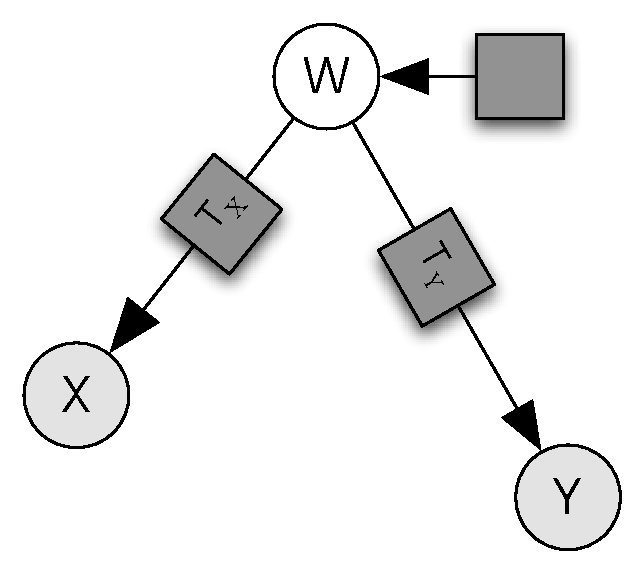
\includegraphics [scale=0.4] {figs/parent.pdf}
  \caption{\figlabel{parent}
    A simple example of transducer composition to build a multi-sequence model of two extant sequences.
    An ancestral sequence $W$ evolves into two descendant sequences $X$ and $Y$.
    A singlet transducer (the horizontal gray box) emit ancestral sequence and structure
    and two branch transducers (the gray boxes labeled $\Delta T_X$ and $\Delta T_Y$)
    mutate it according to the specified multi-sequence model.
    Gray nodes correspond to observed data and white nodes unobserved data.
  }
\end{figure}

Consider the simple model shown in \figref{parent}.
The state of the multi-sequence model describing this model is a 3-vector $\bvec{a} = \left( a_1,\,a_2,\,a_3 \right)$,
where $a_1$ is the state of the singlet transducer generating the ancestral sequence $W$
and $a_2$ and $a_3$ are the states of the branch transducers evolving $W$ into
extant sequences $X$ and $Y$.

We can show some of the allowed transitions of this multi-sequence model.
The state of the branch transducer associated with the active node $n$ is shown in bold.

\paragraph{Stem creation.}

A stem is created at the root node $W$ (corresponding to a bifurcation in the singlet transducer $a_1$)
and survives in the sequence $X$ at node 2 but is deleted in the sequence $Y$ at node 3.

\begin{align}
  \nakedthreevec{1:}{2:}{3:} \quad
  \threevec{L}{L}{\mathbf{L}} &
  \to \threevec{\mathbf{L}}{W_L}{W_L}
  \to \threevec{B}{B}{B_p}
  \to \threevec{L}{L}{\mathbf{L}} \, \threevec{S}{\mathbf{S}}{\Send}
  \to \threevec{L}{L}{\mathbf{L}} \, \threevec{\mathbf{S}}{W_S}{\Send} \\
  & \to \threevec{\mathbf{L}}{W_L}{W_L} \, \threevec{\mathbf{S}}{W_S}{\Send}
\end{align}


\paragraph{Stem insertion.}

A stem sequence is inserted in sequence $X$ at node 2.

\begin{align}
  \nakedthreevec{1:}{2:}{3:} \quad
  \threevec{L}{L}{\mathbf{L}} \to \threevec{L}{\mathbf{L}}{W_L}
  \to \threevec{L}{B_i}{B}
  \to \threevec{L}{L}{\mathbf{L}} \, \threevec{\Send}{S}{\mathbf{S}}
  \to \threevec{\mathbf{L}}{W_L}{W_L} \, \threevec{\Send}{\mathbf{S}}{W_S}
\end{align}

\paragraph{Stem termination.}

All stem sequences are ended by (possibly empty) loop sequences.

\begin{align}
  \nakedthreevec{1:}{2:}{3:} \quad
  \threevec{\mathbf{S}}{W_S}{W_S}
  \to \threevec{B_e}{B_e}{B_e}
  \to \threevec{\Send}{\Send}{\Send} \, \threevec{L}{L}{\mathbf{L}}
  \to \threevec{\Send}{\Send}{\Send} \, \threevec{\Send}{\Send}{\Send}
\end{align}


The functions $\alpha(t)$, $\beta(t)$ and $\gamma(t)$ are parametrized by the insertion and deletion rates of the Structure Tree model.
They are defined for loop sequences as
\begin{align}
  \kappa_1 &= \lambda_1 / \mu_1 \\
  \alpha_1 &= \exp \left( -\mu_1 t \right) \\
  \beta_1 &= \frac{\lambda_1 \left( 1 - \exp \left((\lambda_1 - \mu_1) t \right) \right)}{\mu_1 - \lambda_1 \exp \left( (\lambda_1 - \mu_1) t \right) } \\
  \gamma_1 &= 1 - \frac{\mu_1 \left( 1 - \exp \left((\lambda_1 - \mu_1) t \right) \right)}{\left( 1 - \exp (- \mu_1 t) \right) \left(\mu_1 - \lambda_1 \exp \left( (\lambda_1 - \mu_1) t \right) \right) }
\end{align}
and similarly for stem sequences \cite{Holmes2004}.


\bibliography{../latex-inputs/alignment,../latex-inputs/reconstruction,../latex-inputs/duplication,../latex-inputs/genomics,../latex-inputs/ncrna,../latex-inputs/url}



\end{document}
